%%%%%%%%%%%%%%%%%%%%%%%%%%%%%%%%%%%%%%%%%%%%%%%%%%%%%%%%%%%%%%%%%%%%%%%%%%%%%%%%%%%
% 			Facultad de Ciencias, UAEM.							Agosto de 2013
% 
%	Alumno: 				Emanuel García Perez
%	Asginatura:				Computación y Sociedad
%	Proyecto:				Exposición
%	Tema:					"Censura en Internet // OpenNet Initiative"
%
%%%%%%%%%%%%%%%%%%%%%%%%%%%%%%%%%%%%%%%%%%%%%%%%%%%%%%%%%%%%%%%%%%%%%%%%%%%%%%%%%%%


\documentclass{beamer}

\usepackage[spanish,activeacute]{babel}
\usepackage[latin1]{inputenc}
\usepackage{beamerthemeshadow}
\usepackage{graphicx}

\title{\textbf{Censura en Internet // OpenNet Initiative}}
\author{Emanuel Garc\'ia P\'erez}
\date{\today}

\begin{document}

\frame[allowframebreaks]{\titlepage}
\section[Contenidos]{}
\frame{
\transdissolve[duration=0.2]
\tableofcontents
}


\section{Censura}
\frame
{
\transdissolve[duration=0.2]
\frametitle{?`Qu\'e es la Censura?}
Practica que implica la supresi\'on de contenido de un material de comunicaci\'on por razones ideol\'ogicas, morales o pol\'iticas; cuando cierto contenido es considerado ofensivo, da\~nino, inconveniente o innecesario suele ser censurado por un medio de comunicaci\'on, el gobierno o cualquier otro organismo que as\'i lo determine.
}

\subsection{Justificaciones}
\frame{
\transdissolve[duration=0.2]
\frametitle{Censura Moral}
\begin{figure}
  \centering
    
\includegraphics[width=0.4\textwidth]{cens_1.jpg}
  \label{fig:ejemplo}
\end{figure}
}

\frame{
\transdissolve[duration=0.2]
\frametitle{Censura Militar}
\begin{figure}
  \centering
    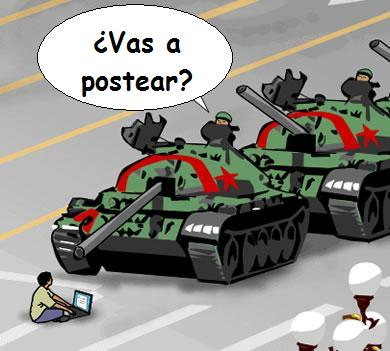
\includegraphics[width=0.6\textwidth]{cens_post.jpg}
  \label{fig:ejemplo}
\end{figure}
}

\frame{
\transdissolve[duration=0.2]
\frametitle{Censura Pol\'itica}
\begin{figure}
  \centering
    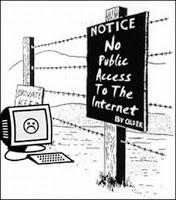
\includegraphics[width=0.5\textwidth]{cens_int.jpg}
  \label{fig:ejemplo}
\end{figure}
}

\frame{
\transdissolve[duration=0.2]
\frametitle{Censura Religiosa}
\begin{figure}
  \centering
    
\includegraphics[width=0.7\textwidth]{cens_4.jpg}
  \label{fig:ejemplo}
\end{figure}
}

\frame{
\transdissolve[duration=0.2]
\frametitle{Censura Corporativa}
\begin{figure}
  \centering
    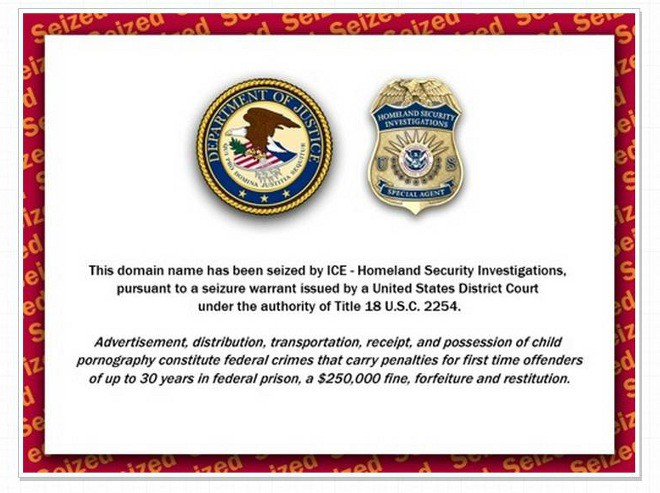
\includegraphics[width=0.7\textwidth]{bloq_int.jpg}
  \label{fig:ejemplo}
\end{figure}
}


\section{Censura en Internet}
\frame
{
\transdissolve[duration=0.2]
\frametitle{?`Qu\'e es la Censura en Internet?}
Todas las normas, t\'ecnicas y m\'etodos que utilizan ciertos grupos y organismos para controlar, manipular y/o suprimir determinados contenidos en Internet.
}

\end{document}
